\documentclass{article}
\title{Project 1}
\author{Nat Hawkins, Victor Ramirez, Mike Roosa, Pranjal Tiwari}
\date{26 Jan, 2017}

\usepackage{relsize,makeidx,color,setspace,amsmath,amsfonts,amssymb}
\usepackage[table]{xcolor}
\usepackage{bm,ltablex,microtype}

\usepackage[top = 1in, bottom = 1in, right = 1in, left = 1in]{geometry}

\usepackage[pdftex]{graphicx}

\begin{document}
\maketitle

\begin{abstract}
	The aim of this project is two-fold: firstly to familiarize ourselves with some computational practices and the use of C++ coding methods (i.e. dynamic memory allocation, compiling of cpp files, etc.) as well as testing the limits of machine accuracy, and second to perform computations using vector and matrix operations in order to solve mathematical problems. We will be comparing the efficiency of use of vectors versus matrices in our solving of these problems.
\end{abstract}
%The above is the abstract. Marked for return to add additional details.

\section{Introduction}
	Before we begin, although C++ will be used for some parts of this project in order to learn the language, the majority of our coding will be done in Python. The three of us have experience in using this language and we decided that it was best to play to our strengths in using the coding language we are most comfortable with. We will do some work with C++ and a discussion of this will be provided in our report. 
	
	\subsection{Mathematical Motivation}
		The motivation behind this project is simple: Many important differential equations in  Science can be written as 	linear second-order differential equations
		\begin{equation*}
		\frac{d^2y}{dx^2}+k^2(x)y = f(x),
		\end{equation*}
		where $f$ is normally called the inhomogeneous term and $k^2$ is a real function.
		
		A classical equation from electromagnetism is Poisson's equation.	The electrostatic potential $\Phi$ is generated by a localized charge distribution $\rho (\mathbf{r})$.   In three dimensions it reads
		
		\begin{equation*}
		\nabla^2 \Phi = -4\pi \rho (\mathbf{r}).
		\end{equation*}
		With a spherically symmetric $\Phi$ and $\rho (\mathbf{r})$  the equations
		simplifies to a one-dimensional equation in $r$, namely
		
		\begin{equation*}
		\frac{1}{r^2}\frac{d}{dr}\left(r^2\frac{d\Phi}{dr}\right) = -4\pi \rho(r),
		\end{equation*}
		which can be rewritten via a substitution $\Phi(r)= \phi(r)/r$ as
		
		\begin{equation*}
		\frac{d^2\phi}{dr^2}= -4\pi r\rho(r).
		\end{equation*}
		The inhomogeneous term $f$ or source term is given by the charge distribution
		$\rho$  multiplied by $r$ and the constant $-4\pi$.
		
		We will rewrite this equation by letting $\phi\rightarrow u$ and 
		$r\rightarrow x$. 
		The general one-dimensional Poisson equation reads then
		
		\begin{equation*}
		-u''(x) = f(x).
		\end{equation*}
		

\section{Solution}
\subsection{Problem Set-Up}
In this project we solved the one-dimensional Poisson equation with Dirichlet boundary conditions by rewriting it as a set of linear equations.

In doing so, our mathematics looked something like the following:

\begin{equation*}
-u''(x) = f(x), \hspace{0.5cm} x\in(0,1), \hspace{0.5cm} u(0) = u(1) = 0.
\end{equation*}

In our case we will assume  that the source term is 
$f(x) = 100e^{-10x}$, and keep the same interval and boundary  conditions. Then the above differential equation
has a closed-form  solution given by $u(x) = 1-(1-e^{-10})x-e^{-10x}$. We will compare
our numerical solution with this result in the future exercise.

We fed the program an input value $i$, which was then used to determine $x$ and the step size $h$. We did this by defining the variables as follows
\begin{equation*}
i = [input], \hspace{0.5cm} n = 10^{i},\hspace{0.5cm}  h = \frac{1.0}{n}
\end{equation*}

We  approximate the second derivative of $u$ with
\begin{equation*}
-\frac{v_{i+1}+v_{i-1}-2v_i}{h^2} = f_i  \hspace{0.5cm} \mathrm{for} \hspace{0.1cm} i=1,\dots, n,
\end{equation*}
where $f_i=f(x_i)$.



We began with a tridiagonal matrix, A, and transformed the problem into the following:

\begin{equation*}
\mathbf{A}\mathbf{v} = \tilde{\mathbf{b}},
\end{equation*}
where $\mathbf{A}$ is an $n\times n$  tridiagonal matrix which we rewrite as

\[
\mathbf{A} = \begin{bmatrix}
2& -1& 0 &\dots   & \dots &0 \\
-1 & 2 & -1 &0 &\dots &\dots \\
0&-1 &2 & -1 & 0 & \dots \\
& \dots   & \dots &\dots   &\dots & \dots \\
0&\dots   &  &-1 &2& -1 \\
0&\dots    &  & 0  &-1 & 2 \\
\end{bmatrix},
\]
and $\tilde{b}_i=h^2f_i$.  A can be derived by looking at the formula for the approximation of the second derivative. Note how the $v_{i+1}$ and the $v_{i-1}$ terms have a coefficient of $-1$. This is where the off diagonal elements come from in our matrix A. Since the two off diagonal entries are equivalent, we can approximate them into one vector, $e$. However, since all of the entries are -1, we decided to not allocate memory to this. Instead, we simplified our algorithm to account for these values. We will discuss our problem solving algorithms in the following section.

The reason for the conversion from a matrix to vectors comes about in our number of floating point operations (FLOPS). In using the matrix approximation, we were looking at (reference) $~\frac{2}{3}n^{3}$ FLOPS in calculating our solutions. However, in being able to reduce this down to a vector problem, we managed to reduced our calculations to $9n$, and then further to $4n$, again to be discussed in the next section. The short of this discussion is that we were able to reduce our floating point operations by two orders of magnitude. In the sense of computational efficiency, this makes for much smarter problem solving and much more effective computation. 

\subsection{Algorithms}
The algorithms that we implemented in the solving of this problem are as follows. We denote the dioagonal elements as $d[i]$, the solution values as $u[i]$, and the values of the function as $f[i]$. The problem starts when look at a general case for a $4x4$ matrix:

\[
\mathbf{A} = \begin{bmatrix}
d_{1}& e_{1}& 0& 0& \\
e_{1}& d_{2}& e_{2}& 0& \\
0& e_{2}& d_{3}& e_{3}& \\
0& 0& e_{3}& d_{4}& \\

\end{bmatrix},
\]

\[
\mathbf{u} = \begin{bmatrix}
u_{1}\\
u_{2} \\
u_{3}\\
u_{4}\\
\end{bmatrix},
\]

\[
\mathbf{f} = \begin{bmatrix}
f_{1}\\
f_{2} \\
f_{3}\\
f_{4}\\
\end{bmatrix},
\]

And now we can look at solving $\mathbf{A}\mathbf{u} = \tilde{\mathbf{f}},$ through the process of Gaussian Elimination. For this process, reference (reference). In essence, we begin by multiplying the second row of $A$ by the ratio of the terms in the first column of rows one and two. Explicitly, this looks like $\frac{e_{1}}{d_{1}}$ on both the right hand side and left hand side. This transforms the equation into the following: 

\[
\begin{Bmatrix}
d_{1}& e_{1}& 0& 0& \\
0& d_{2}-\frac{e_{1}^{2}}{d_{1}}& e_{2}& 0& \\
0& e_{2}& d_{3}& e_{3}& \\
0& 0& e_{3}& d_{4}& \\
\end{Bmatrix}
*
\begin{Bmatrix}
content...
\end{Bmatrix}
\]

\subsection{Problem 1c}

\subsection{Relative Error}
We calculated the relative error in the data set $i=1,\dots, n$,by setting up

\[
\epsilon_i=log_{10}\left(\left|\frac{v_i-u_i}
{u_i}\right|\right),
\]
as function of $log_{10}(h)$ for the function values $u_i$ and $v_i$.
For each step length, we saw that the error was pretty much a constant value. That meaning that for each value of $x$, the relative error was approximately the exact same. Since the error was the exact same for all x values, we elected to choose only one points error from each trial. However, we elected to choose the first value in each trial for our error (i.e. $i=1, x= 0.1 \hspace{0.5cm} i=2, x = 0.01, etc.$). We were consistent with our choice, so whatever error that this may have imposed, we were at least consistent with this. We then conducted multiple trials utilizing values of $i$ ranging from $i=0$ to $i=8$. The results we got are below:

\begin{figure}[h!]
	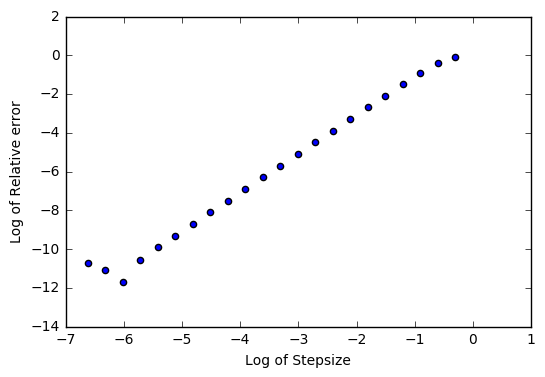
\includegraphics[width=\linewidth]{PHY480_P1_RerrvSs.png}
	\caption{Plot of Log of Relative Error. On the x-axis, we see the log of the step-size. This is equivalent to looking at which $i$ value we chose to use in order to approximate our solution. The y-axis shows the log of the relative error given in the equation above. What we see is that the log of error has a slope of approximately -2, as expected in our initial mathematic discussion. The error begins to increase again after $i=6$ or $n=10^{6}, h \approx 10^{-6}$. This is due to the truncation error that is getting overwritten by the number of bits. The increase in error can be accounted to machine error.}
	\label{fig:errorplot}
\end{figure}


\subsection{Problem 1e}


\end{document}